\chapter{The 2018 project}
\label{chap:legacy}

In 2018 we built two things: a segmentation of the slices in Matlab, and a Python application that
turned its masks into a 3D model. This chapter summarises both, then looks back at their limitations.
The masks our segmentation produced on the reference stack serve as the 2018 baseline in the rest of
this report.

\section{The brief}

The laboratory's brief listed six goals: be compatible with the laboratory's tools (Windows, ImageJ,
CTan); threshold the vascular network apart from the bone; reconstruct and improve the continuity of
the network; build the tools needed to quantify it (nodes, branches, vessel size, branch length);
study the inter- and intra-sample reproducibility; automate the measurements.

\section{Segmentation (Matlab)}

We weighed machine learning against mathematical morphology. Machine learning could learn subjective
criteria, but needed a large labelled database that the researchers would have had to build;
morphology was quick to set up and gave immediate results. We chose morphology, developed in Matlab,
in three versions.

\paragraph{Version 1: thresholds} The 16-bit histogram shows distinct modes
(Figure~\ref{fig:legacy-histogram}). A two-level Otsu threshold (\code{multithresh}), computed
\emph{for each slice}, split the image into background, bone and bright contrast agent. The bone and
the burst clusters were cleanly separated, but many vessels were still counted as bone.

\paragraph{Version 2: openings and closings} Connected components larger than 700 pixels were
declared bone; smaller foreground blobs became ``dark'' vessels. Burst clusters were searched among the
bright pixels: dilated bright regions larger than 1000 pixels with a squarish bounding box, plus dark
regions found by adaptive binarisation and kept if their intensity standard deviation exceeded 2500,
then closed, dilated and reconstructed with disks of 5 to 15 pixels. The researchers approved this
segmentation, while acknowledging ``zones of uncertainty'' between vessels and trabeculae.

\paragraph{Version 3: slice-to-slice connectivity} Each slice was corrected with its two neighbours,
a three-slice majority vote: a pixel set in slices $n-1$ and $n+1$ but not in $n$ was added
($101 \rightarrow 111$), an isolated one removed ($010 \rightarrow 000$). The masks of bone and
vessels were written as PNG images, one pair per slice; bursts were discarded.

\begin{figure}[ht]
  \centering
  \begin{subfigure}[t]{0.32\linewidth}\centering
    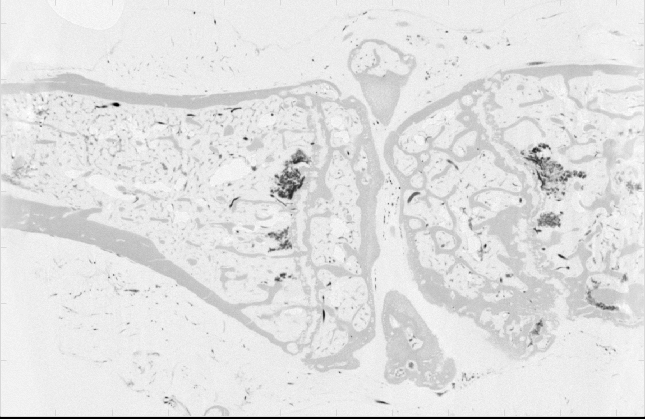
\includegraphics[angle=-90,width=\linewidth]{original.png}\caption{Original slice.}
  \end{subfigure}\hfill
  \begin{subfigure}[t]{0.32\linewidth}\centering
    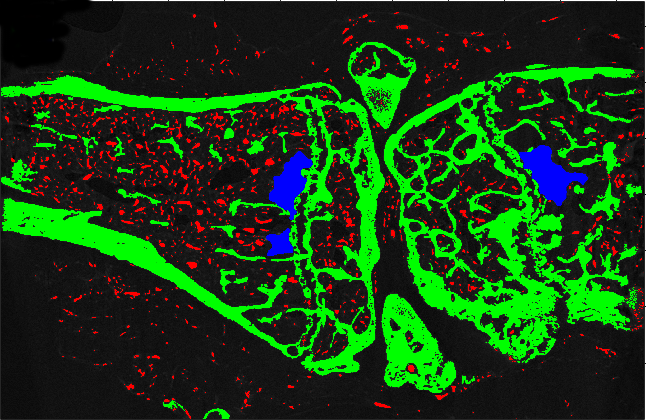
\includegraphics[angle=-90,width=\linewidth]{results2.png}\caption{Version 2.}
  \end{subfigure}\hfill
  \begin{subfigure}[t]{0.32\linewidth}\centering
    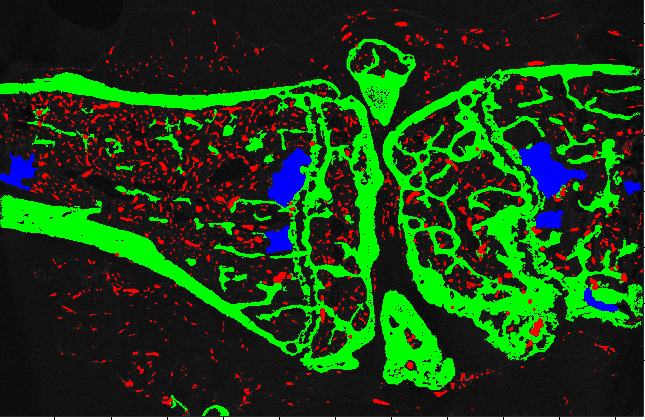
\includegraphics[angle=-90,width=\linewidth]{results3.png}\caption{Version 3.}
  \end{subfigure}
  \caption{Our 2018 segmentation, in the colours we used then: bone in green, vessels in red, burst
    clusters in blue.}
  \label{fig:legacy-results}
\end{figure}

\begin{figure}[ht]
  \centering
  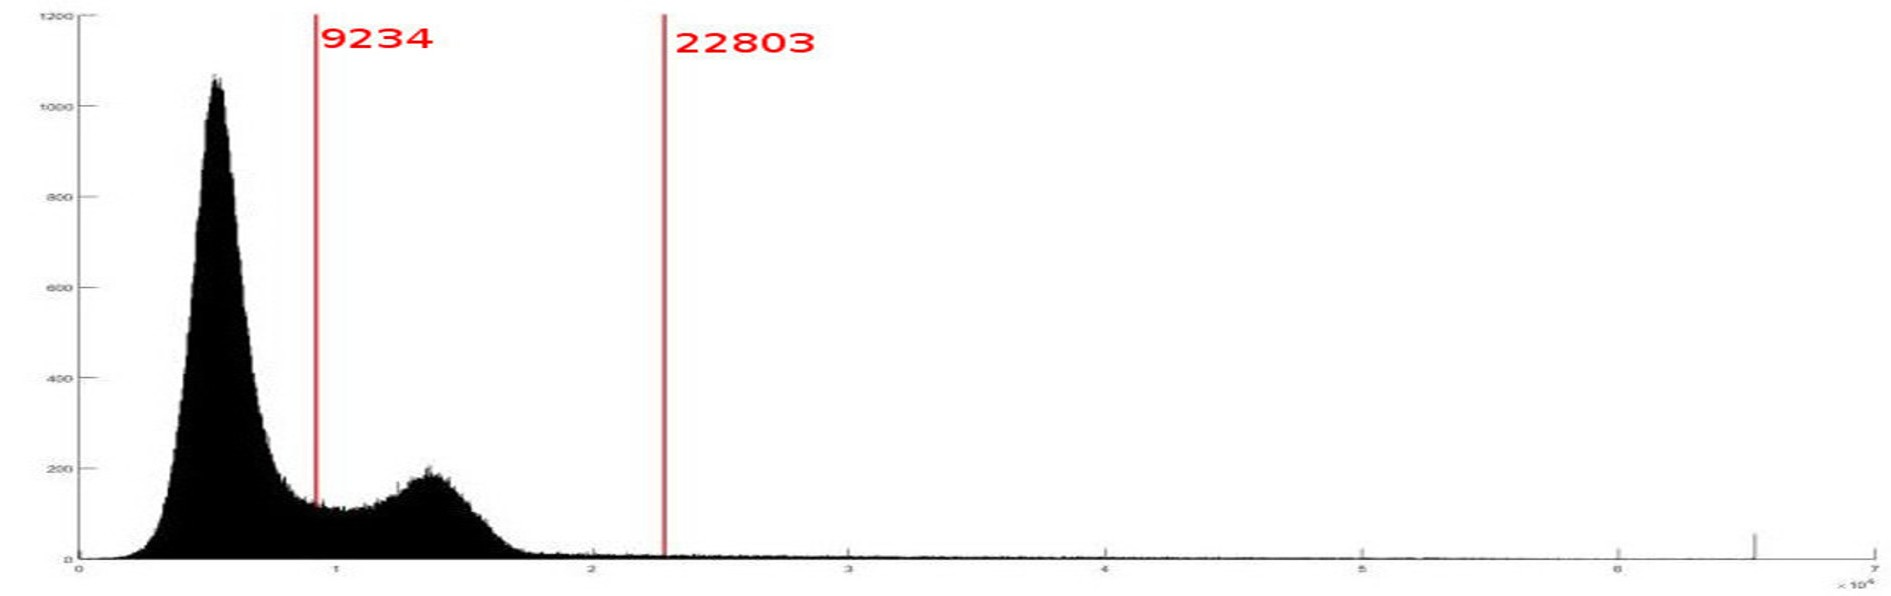
\includegraphics[width=0.7\linewidth]{histogrammeshort.jpg}
  \caption{Histogram of one slice (2018 figure): its modes motivated the multi-level threshold.}
  \label{fig:legacy-histogram}
\end{figure}

\section{3D modelling (Python, PyQt5)}

The second half of the project turned the masks into a 3D model. Our PyQt5 application let the user pick
a folder of masks, enter the physical dimensions and a ``marching cube accuracy'' between 1 and 50
(the step of the algorithm), then: stack the PNG masks into a Matlab \code{.mat} volume; run the
Lewiner marching cubes of scikit-image; either display the mesh with matplotlib's
\code{Poly3DCollection}, or save it as an STL file, checked on an online viewer
(Figure~\ref{fig:legacy-modelling}). We had already noted at the time that the matplotlib rendering was
slow, memory-hungry and badly scaled, that the STL showed the ``cubic aspect'' of marching cubes, and
that the program needed a lot of memory. Chapter~\ref{chap:rewrite} describes what replaces it today:
a web page drawing smoothed meshes on the graphics card.

\begin{figure}[ht]
  \centering
  \begin{subfigure}[t]{0.32\linewidth}\centering
    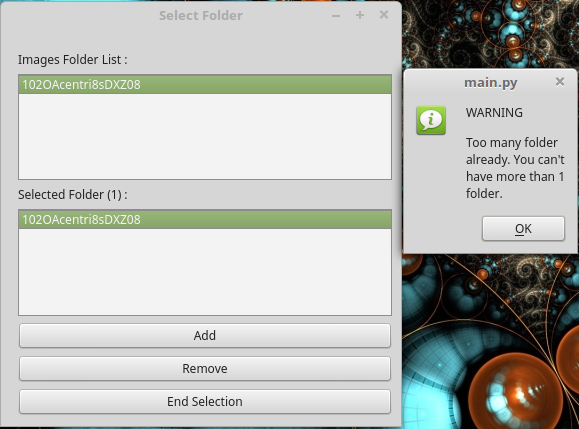
\includegraphics[height=4cm,width=\linewidth,keepaspectratio]{IHM02.png}
    \caption{PyQt5 interface.}
  \end{subfigure}\hfill
  \begin{subfigure}[t]{0.32\linewidth}\centering
    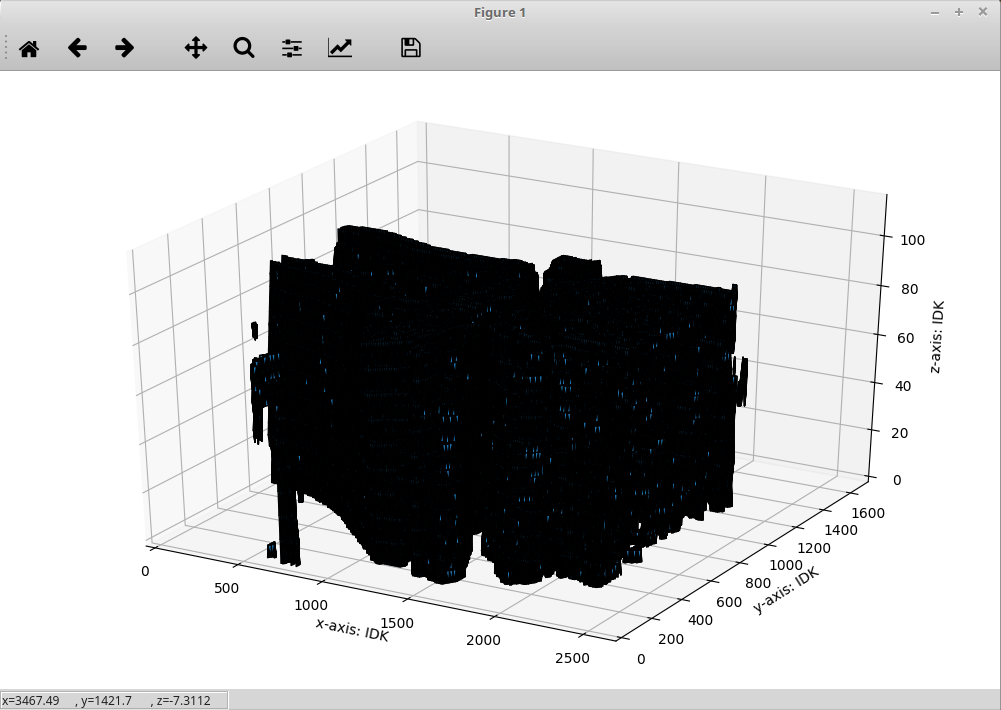
\includegraphics[height=4cm,width=\linewidth,keepaspectratio]{Plot3D01.png}
    \caption{Matplotlib rendering.}
  \end{subfigure}\hfill
  \begin{subfigure}[t]{0.32\linewidth}\centering
    \raisebox{\depth}{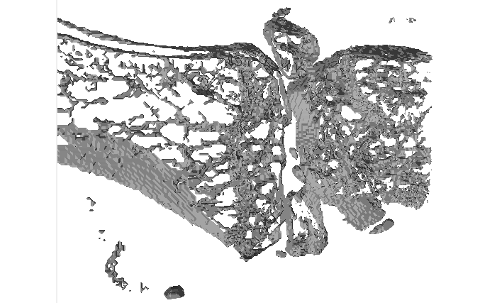
\includegraphics[angle=-90,totalheight=4cm,width=\linewidth,keepaspectratio]{STL01.png}}
    \caption{STL in a viewer.}
  \end{subfigure}
  \caption{The 2018 modelling application.}
  \label{fig:legacy-modelling}
\end{figure}

\section{Limitations}

Looking back with the data at hand, our project had the merit of working end to end in a few weeks,
and of identifying the real difficulty (vessels versus trabeculae). Its limitations fall into three
groups.

\paragraph{Method}
\begin{itemize}
  \item \textbf{Hand-tuned pixel counts.} We tuned every parameter (700 pixels, disks of 5 to 15
        pixels, a standard deviation of 2500 grey levels) on this scan, in pixels. At another
        resolution, or on another animal, none of them keeps its meaning.
  \item \textbf{Per-slice thresholds.} Each slice got its own Otsu thresholds, so the same tissue
        could change class from one slice to the next.
  \item \textbf{Vessel size.} The vessel masks are much thicker than the vessels: their boundary was
        set by morphology, not by the physics of the image (Section~\ref{sec:edges} measures it).
  \item \textbf{Ambiguous blobs.} Every small bone-intensity blob became a vessel. Some are
        dim (clotted) vessels, others are cross-sections of trabecular rods: a 2D slice cannot tell.
  \item \textbf{Bursts discarded} rather than delineated, and \textbf{thin structures eroded} by the
        three-slice vote, which deletes anything only one slice thick.
\end{itemize}

\paragraph{Engineering} The pipeline needed Matlab, exchanged hundreds of intermediate PNG and
\code{.mat} files, hard-coded its paths, held whole volumes in memory, and had no tests.

\paragraph{Validation} Apart from the researchers' visual approval, nothing measured the quality of the
segmentation, so we could not show that any change was an improvement. We did not reach the
quantification goals of the brief.
